% ====================================================================
%  RQ2 -- Competing risks and multiple events (Chapter 4, ~10 min)
%  Layout convention: text/maths left, figure right.
%  Wide multi-panel figures are shown full width with text above.
% ====================================================================

\roadmapframe{2}{RQ2. How can a single survival model predict the time to multiple events that may be competing or co-occurring, and use temporal ordering information when available?}

\begin{frame}{One survival curve per event, per patient}
\begin{columns}[c]
  \begin{column}{0.42\textwidth}
    \small
    Data with $K$ events and right-censoring:
    \[
      \D = \big\{(\bm{x}^{(i)}, \bm{t}^{(i)}, \bm{\delta}^{(i)})\big\}_{i=1}^{N}
    \]
    \[
      \bm{t}^{(i)} \in \R_{+}^{K}, \quad \bm{\delta}^{(i)} \in \{0,1\}^{K}
    \]
    Predict, for each patient,
    \[
      \hat{\bm{S}}^{(i)} = \big[\hat S_1(t \mid \bm{x}^{(i)}), \dots, \hat S_K(t \mid \bm{x}^{(i)})\big]
    \]
    \vspace{-0.5em}
    \begin{itemize}
      \item One model per event ignores shared structure and event order
      \item \dots\ and the cost grows with $K$.
    \end{itemize}
  \end{column}
  \begin{column}{0.56\textwidth}
    \centering
    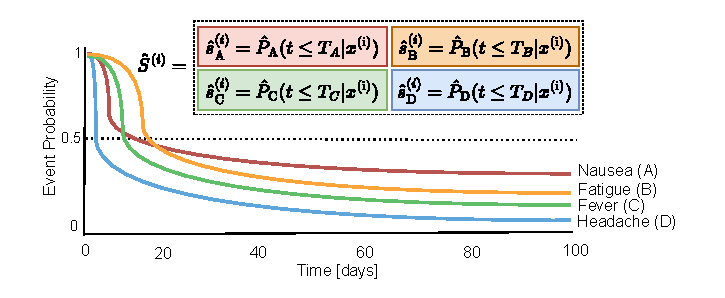
\includegraphics[width=\linewidth, trim=10 0 10 0, clip]{mensa_multi_event.pdf}
    \figsource{Figure from Lillelund et al.~\cite{lillelund_mensa_2026}}
  \end{column}
\end{columns}
\end{frame}

\begin{frame}{MENSA: shared network, Weibull mixtures}
\small
A shared MLP learns a common representation $\tilde{\bm{x}}$; event-specific layers turn it into one \textbf{mixture of Weibulls} per event -- closed-form $f$ and $S$, and fewer parameters than one model per event.
\vspace{0.3em}
\begin{center}
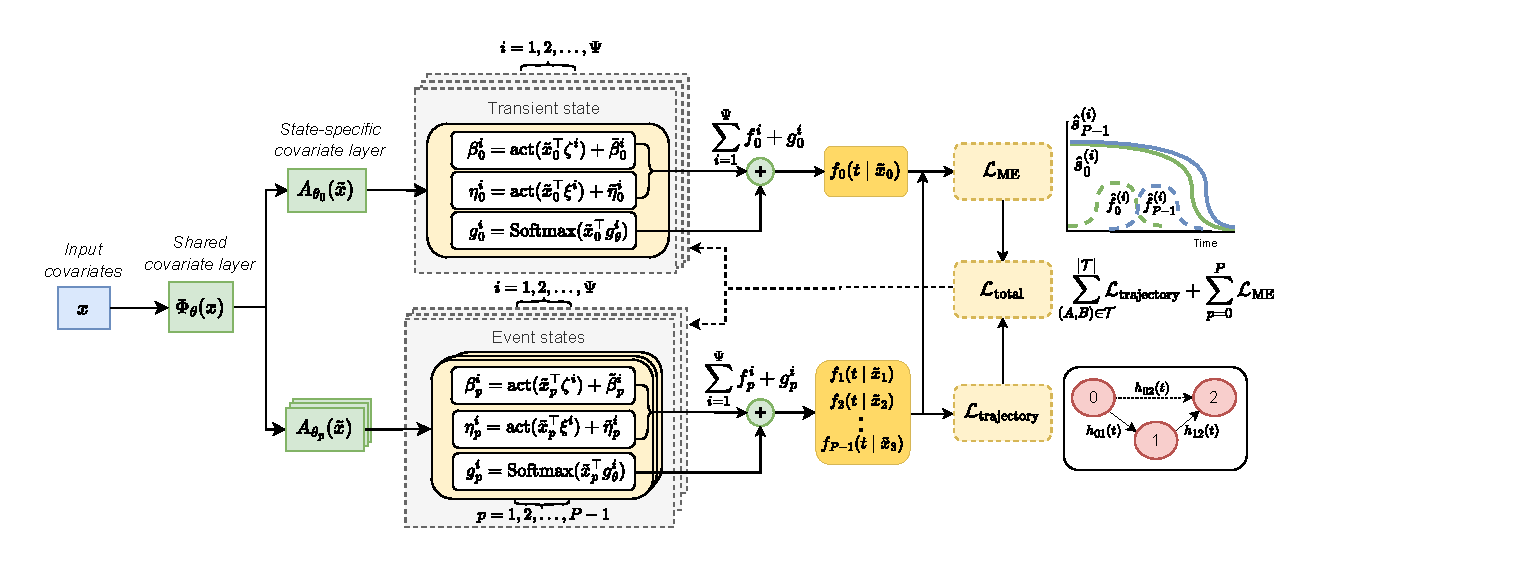
\includegraphics[trim={15 10 108 10},clip,width=\linewidth,height=0.72\textheight,keepaspectratio]{mensa_architecture.pdf}
\end{center}
\vspace{-0.6em}
\figsource{Figure from Lillelund et al.~\cite{lillelund_mensa_2026}}
\end{frame}

\begin{frame}{Using event order: trajectory likelihood}
\begin{columns}[c]
  \begin{column}{0.68\textwidth}
    \footnotesize
    \textbf{Multi-event likelihood} (censoring handled per event):
    \[
      \mathcal{L}_{\text{ME}} = \sum_{i=1}^{N} \sum_{p} w_p
      \Big[\delta_p^{(i)} \log f_p(t_p^{(i)}) + \big(1 - \delta_p^{(i)}\big) \log S_p(t_p^{(i)})\Big]
    \]
    \textbf{Trajectory term:} if $A$ must come before $B$ (e.g.\ relapse $\to$ death),
    \[
      \mathcal{L}_{\text{traj}} = \sum_{i=1}^{N} \sum_{(A,B)}
      \delta_A^{(i)} \delta_B^{(i)} \log S_B\big(t_A^{(i)} \mid \bm{x}^{(i)}\big)
    \]
    $\Rightarrow$ $B$ should still be unlikely at the time $A$ happens.
    \[
      \mathcal{L} = (1 - \lambda)\, \mathcal{L}_{\text{ME}} + \lambda\, \mathcal{L}_{\text{traj}}
    \]
  \end{column}
  \begin{column}{0.3\textwidth}
    \centering
    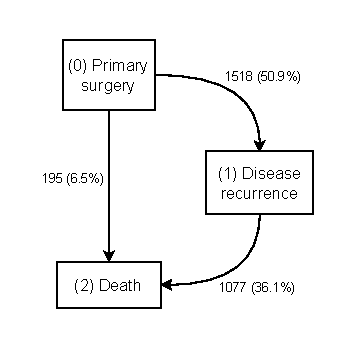
\includegraphics[width=\linewidth, trim=10 10 10 10, clip]{rotterdam.pdf}
    \figsource{Figure from Lillelund et al.~\cite{lillelund_mensa_2026}. Event trajectories in Rotterdam ($N = 2{,}982$).}
  \end{column}
\end{columns}
\end{frame}

\begin{frame}{MENSA: competitive and stable}
\small 4 multi-event datasets, 10 baselines incl.\ DeepHit \cite{lee_deephit_2018} and Hierarchical \cite{tjandra_hierarchical_2021}, 10 runs.
\vspace{0.1em}

\centering
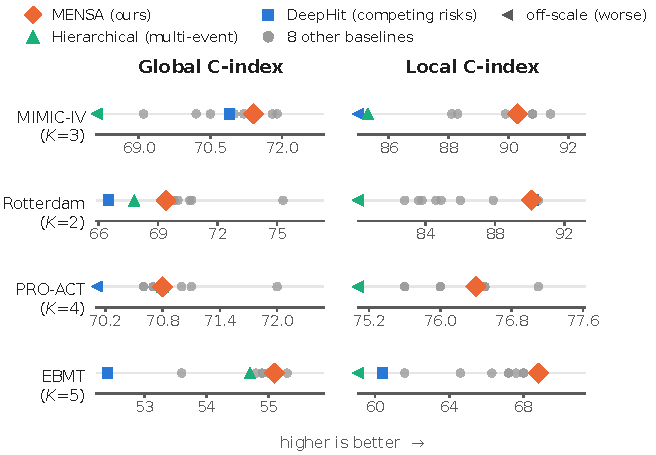
\includegraphics[width=0.74\linewidth]{plot_mensa_results.pdf}
\figsource{Data from Lillelund et al.~\cite{lillelund_mensa_2026}. Global CI ranks patients; local CI ranks events within a patient.}
\takeaway{Top group on both C-indices.}
\end{frame}

\begin{frame}{Ablations: both components help}
\begin{columns}[c]
  \begin{column}{0.44\textwidth}
    \small
    \begin{itemize}
      \item \textbf{Joint training}: within-patient ordering improves -- 90.2 vs.\ 87.8 on Rotterdam.
      \item Independent training is slightly better on \emph{global} metrics.
      \item \textbf{Trajectory loss}: small gains in local CI on Rotterdam and EBMT -- small relative to run-to-run variability.
    \end{itemize}
  \end{column}
  \begin{column}{0.54\textwidth}
    \centering
    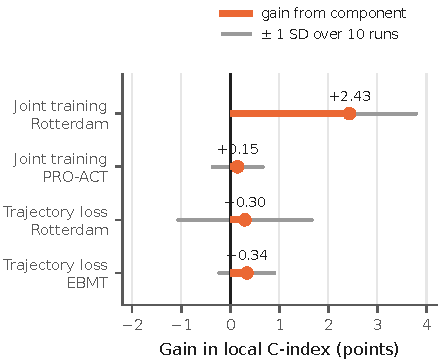
\includegraphics[width=\linewidth]{plot_mensa_ablation.pdf}
    \figsource{Data from Lillelund et al.~\cite{lillelund_mensa_2026}}
  \end{column}
\end{columns}
\end{frame}

% ------------------------------------------------------------------ ALS
\begin{frame}{ALS: when will each function be lost?}
\small
\textit{``How much longer will I be able to speak clearly enough to be understood?''}
\vspace{0.2em}
\begin{columns}[T]
  \begin{column}{0.5\textwidth}
    \begin{itemize}
      \item PRO-ACT \cite{atassi_proact_2014}: 3,220 patients, 8 covariates
      \item Event $k$: ALSFRS-R item $\le 2$, within 500 days
    \end{itemize}
  \end{column}
  \begin{column}{0.48\textwidth}
    \begin{itemize}
      \item $K = 5$: Speech, Swallowing, Handwriting, Walking, Dyspnea
      \item Distinct events, \emph{not} mutually exclusive
    \end{itemize}
  \end{column}
\end{columns}
\begin{center}
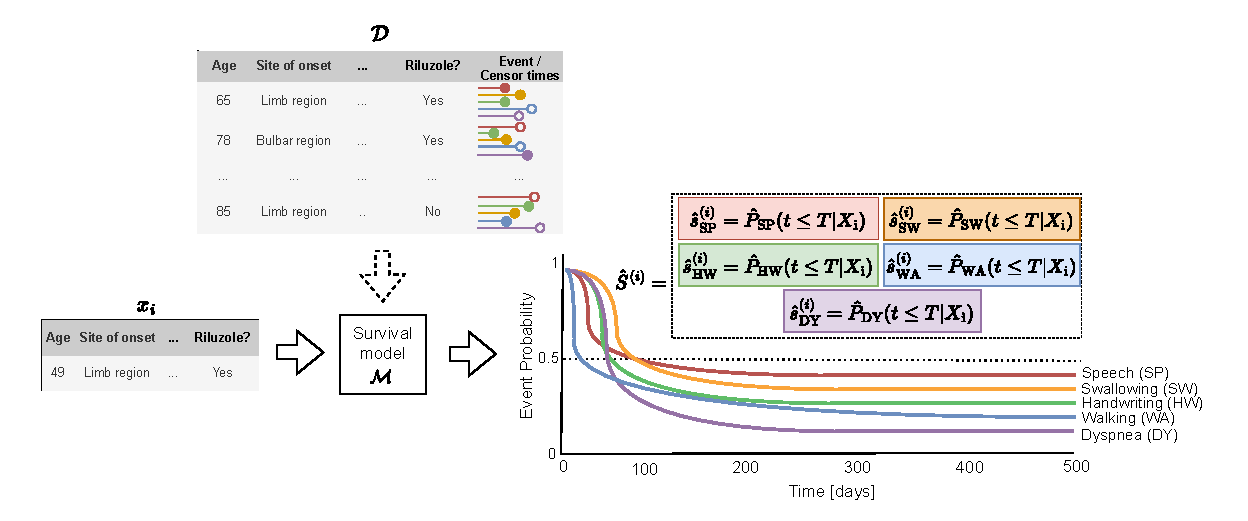
\includegraphics[width=0.86\linewidth]{als_model.pdf}
\end{center}
\vspace{-0.6em}
\figsource{Figure from Lillelund et al.~\cite{lillelund_meaningful_2025}}
\end{frame}

\begin{frame}{Better than the population estimate}
\small Error in days; censored patients get their \emph{margin time} (RQ3):
\[
  \text{mMAE} = \tfrac{1}{N}\textstyle\sum_{i} \big|\tilde e_i - \hat e_i\big|, \qquad
  \tilde e_i = e_i \text{ if } \delta_i = 1, \text{ else } e^{\text{margin}}_i
\]
\vspace{-1.2em}
\begin{center}
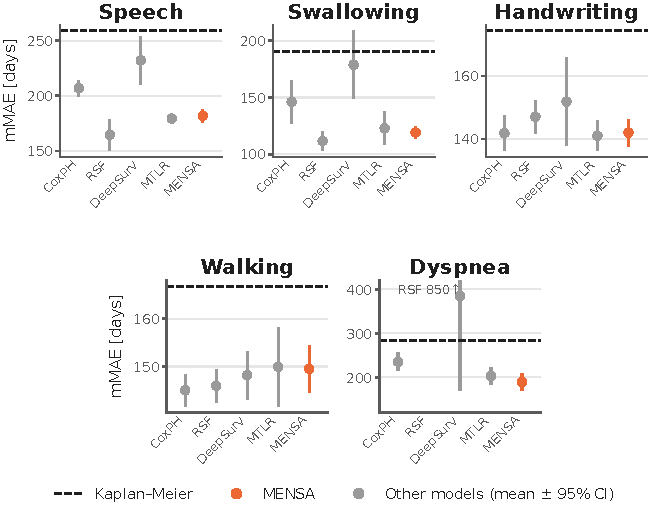
\includegraphics[width=0.66\linewidth]{plot_als_model_vs_km.pdf}
\end{center}
\vspace{-0.9em}
\figsource{Data from Lillelund et al.~\cite{lillelund_meaningful_2025}. Lower is better.}
\end{frame}

\begin{frame}{What if? Site of onset}
\small Change one covariate, recompute all five curves (the paper also shows Riluzole, FVC and baseline ALSFRS-R). \textbf{Bulbar vs.\ limb onset}: bulbar moves Speech and Swallowing decline earlier; the other three change less.
\vspace{-0.4em}
\begin{center}
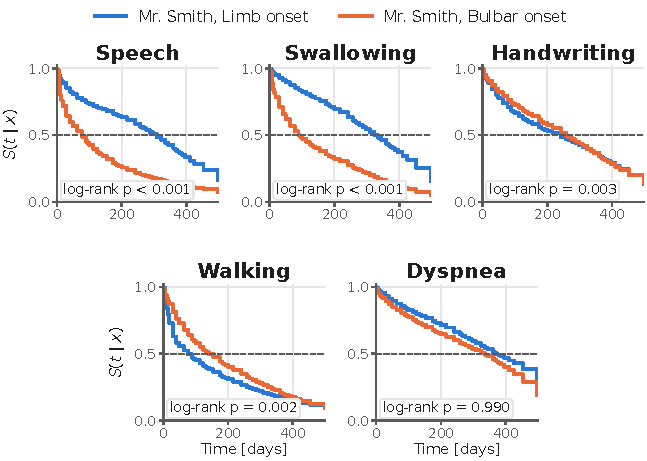
\includegraphics[width=0.74\linewidth]{plot_als_cf_onset.pdf}
\end{center}
\vspace{-0.9em}
\figsource{Data from Lillelund et al.~\cite{lillelund_meaningful_2025}}
\end{frame}

